\subsection{High Threshold Cherenkov Counter (HTCC)}

\subsubsection{Geometry}

The HTCC geometry is implemented through the native GEMC geometry API. The elliptical mirrors are subtractions of
ellipsoid Geant4 volumes along certain planes between two adjacent mirror substrates. Each plane is defined by a second order
curve along which the two substrates intersect.
They are contained inside an HTCC mother volume made with a Geant4 ``polycone'' (\F{htccGeometry}).
The faces of the PMTs are the sensitive volumes, associated with the quartz-glass material and with the HTCC digitization routine.

The refractive index of the $CO_2$ radiator gas and its transparency is included in the material optical properties and taken
into account during the Geant4 transportation of the photons. The same is true for the reflectivity of the mirrors and Winston cones.
Finally, the quantum efficiency associated with the PMT photocathode is taken into account in
the digitization routine.


\begin{figure}
	\centering
	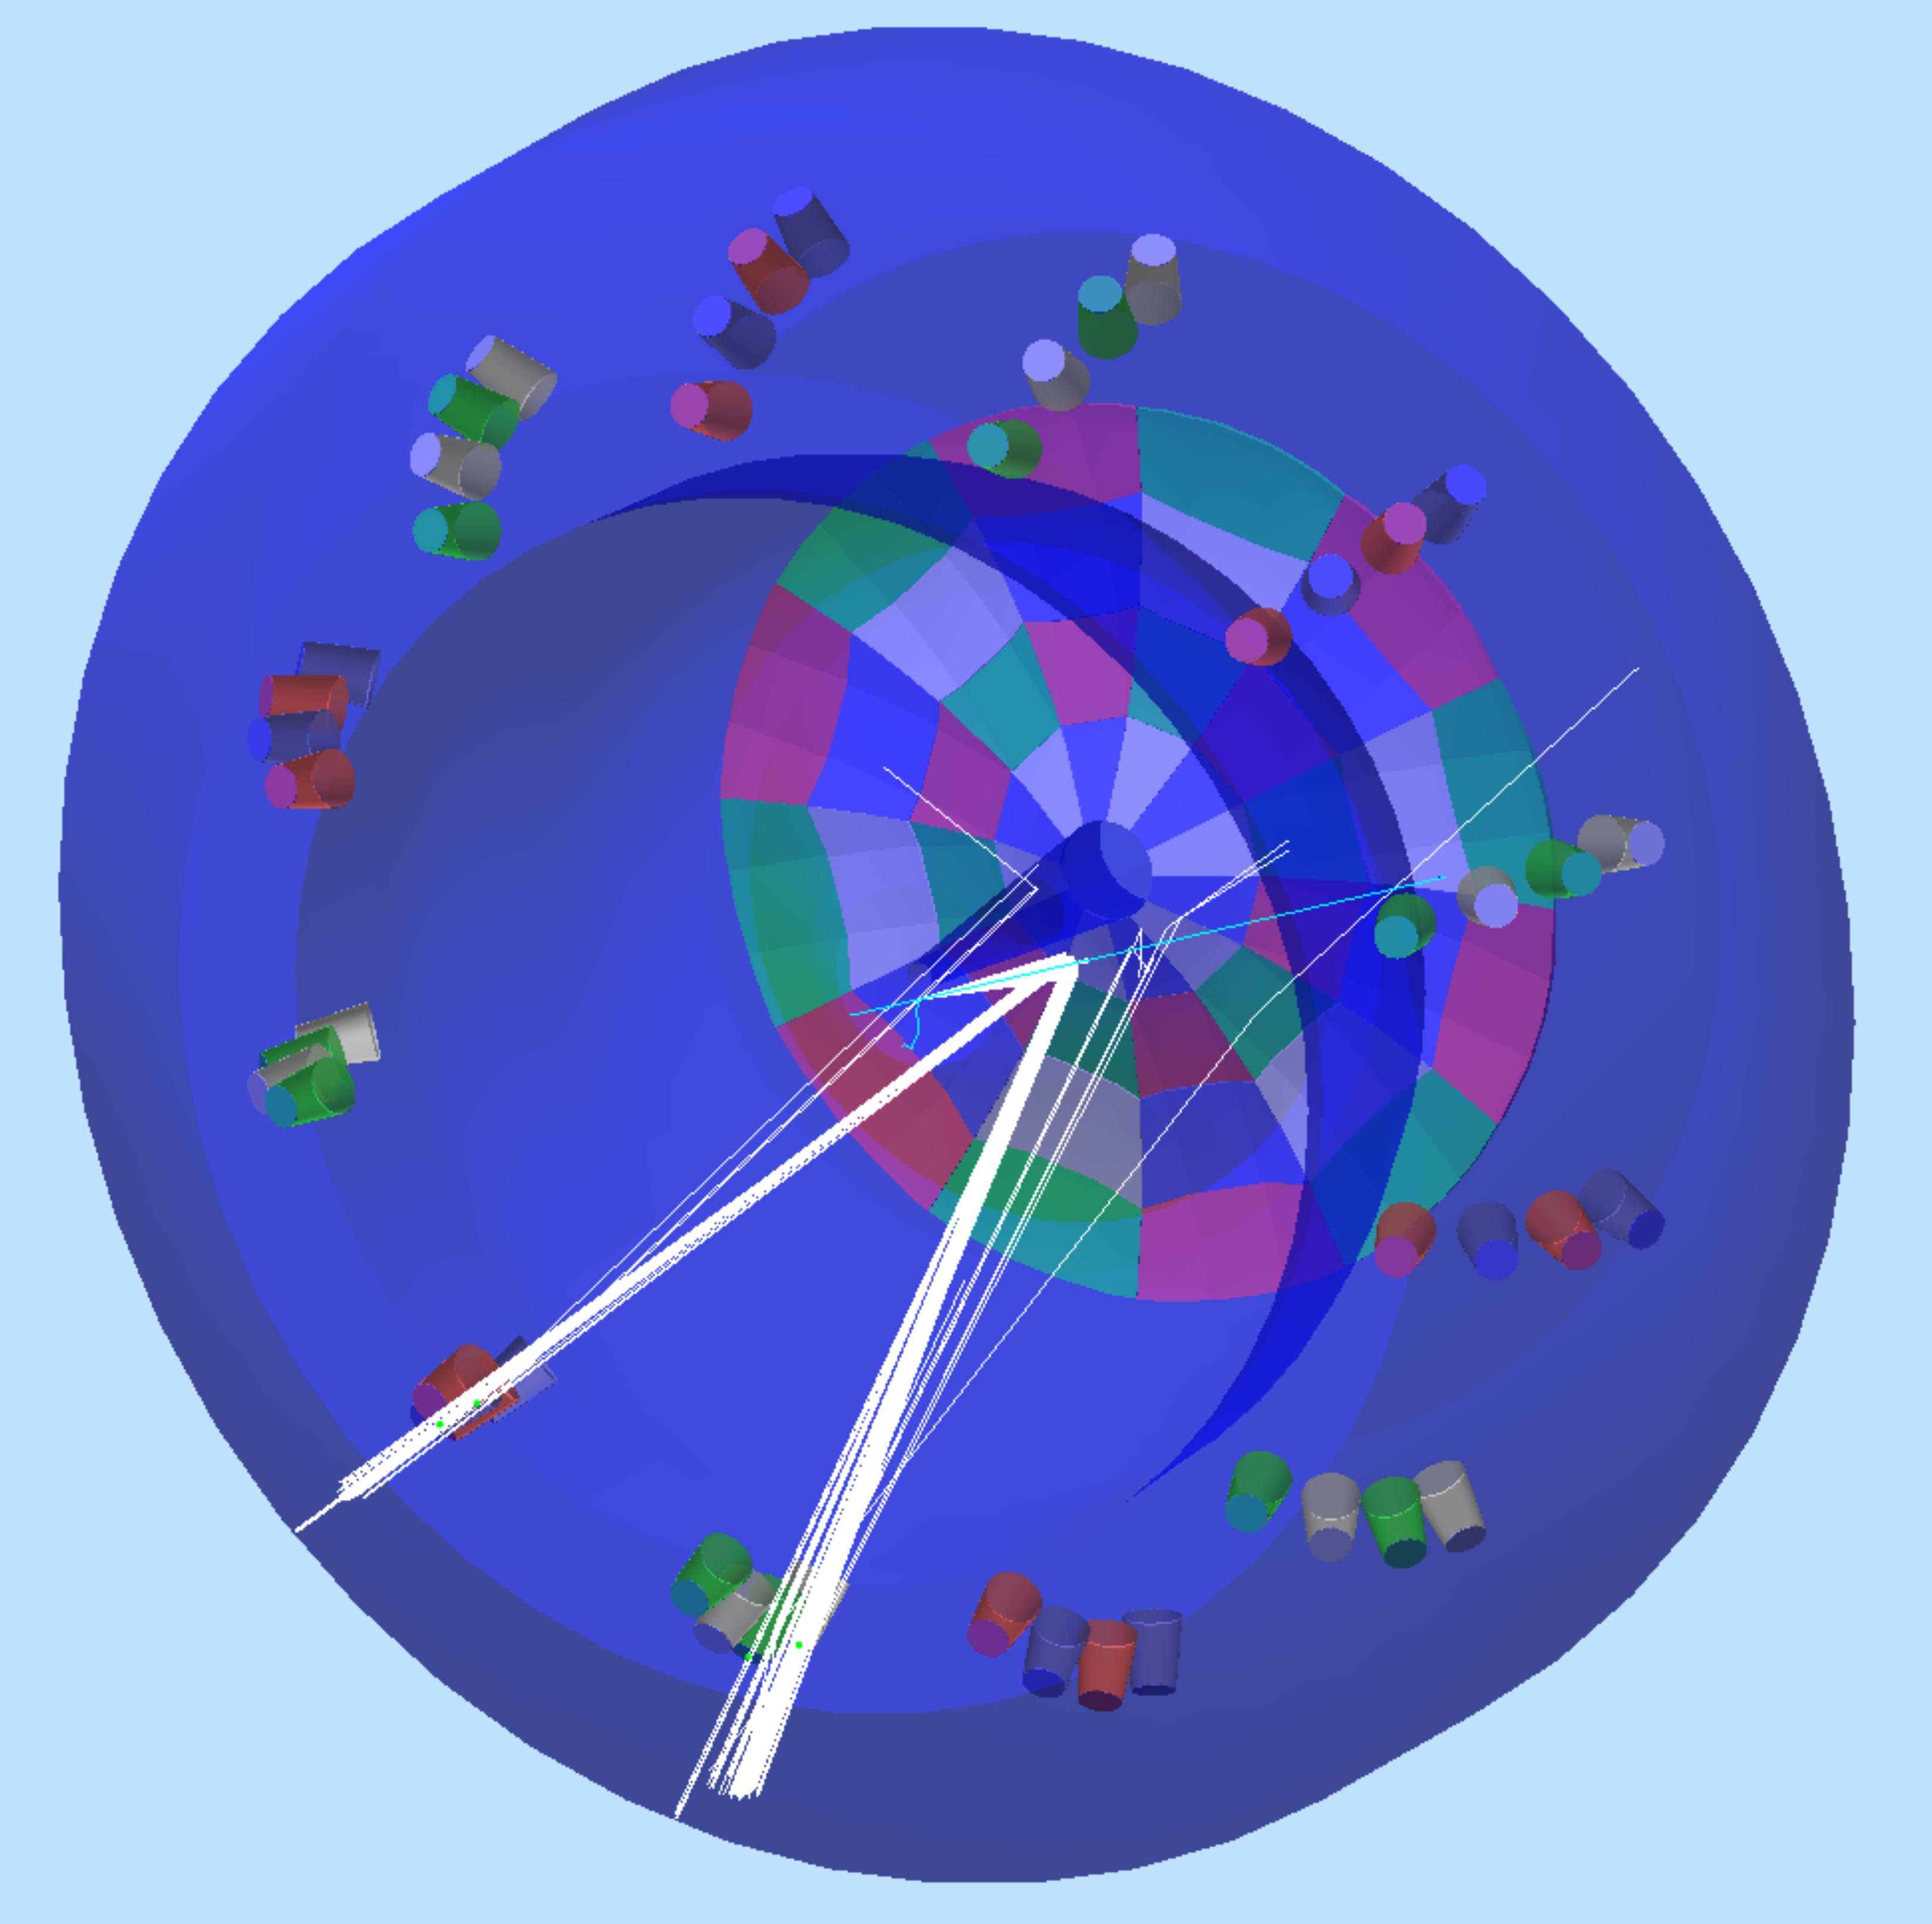
\includegraphics[width=0.99\columnwidth,keepaspectratio]{img/htccGeometry.png}
	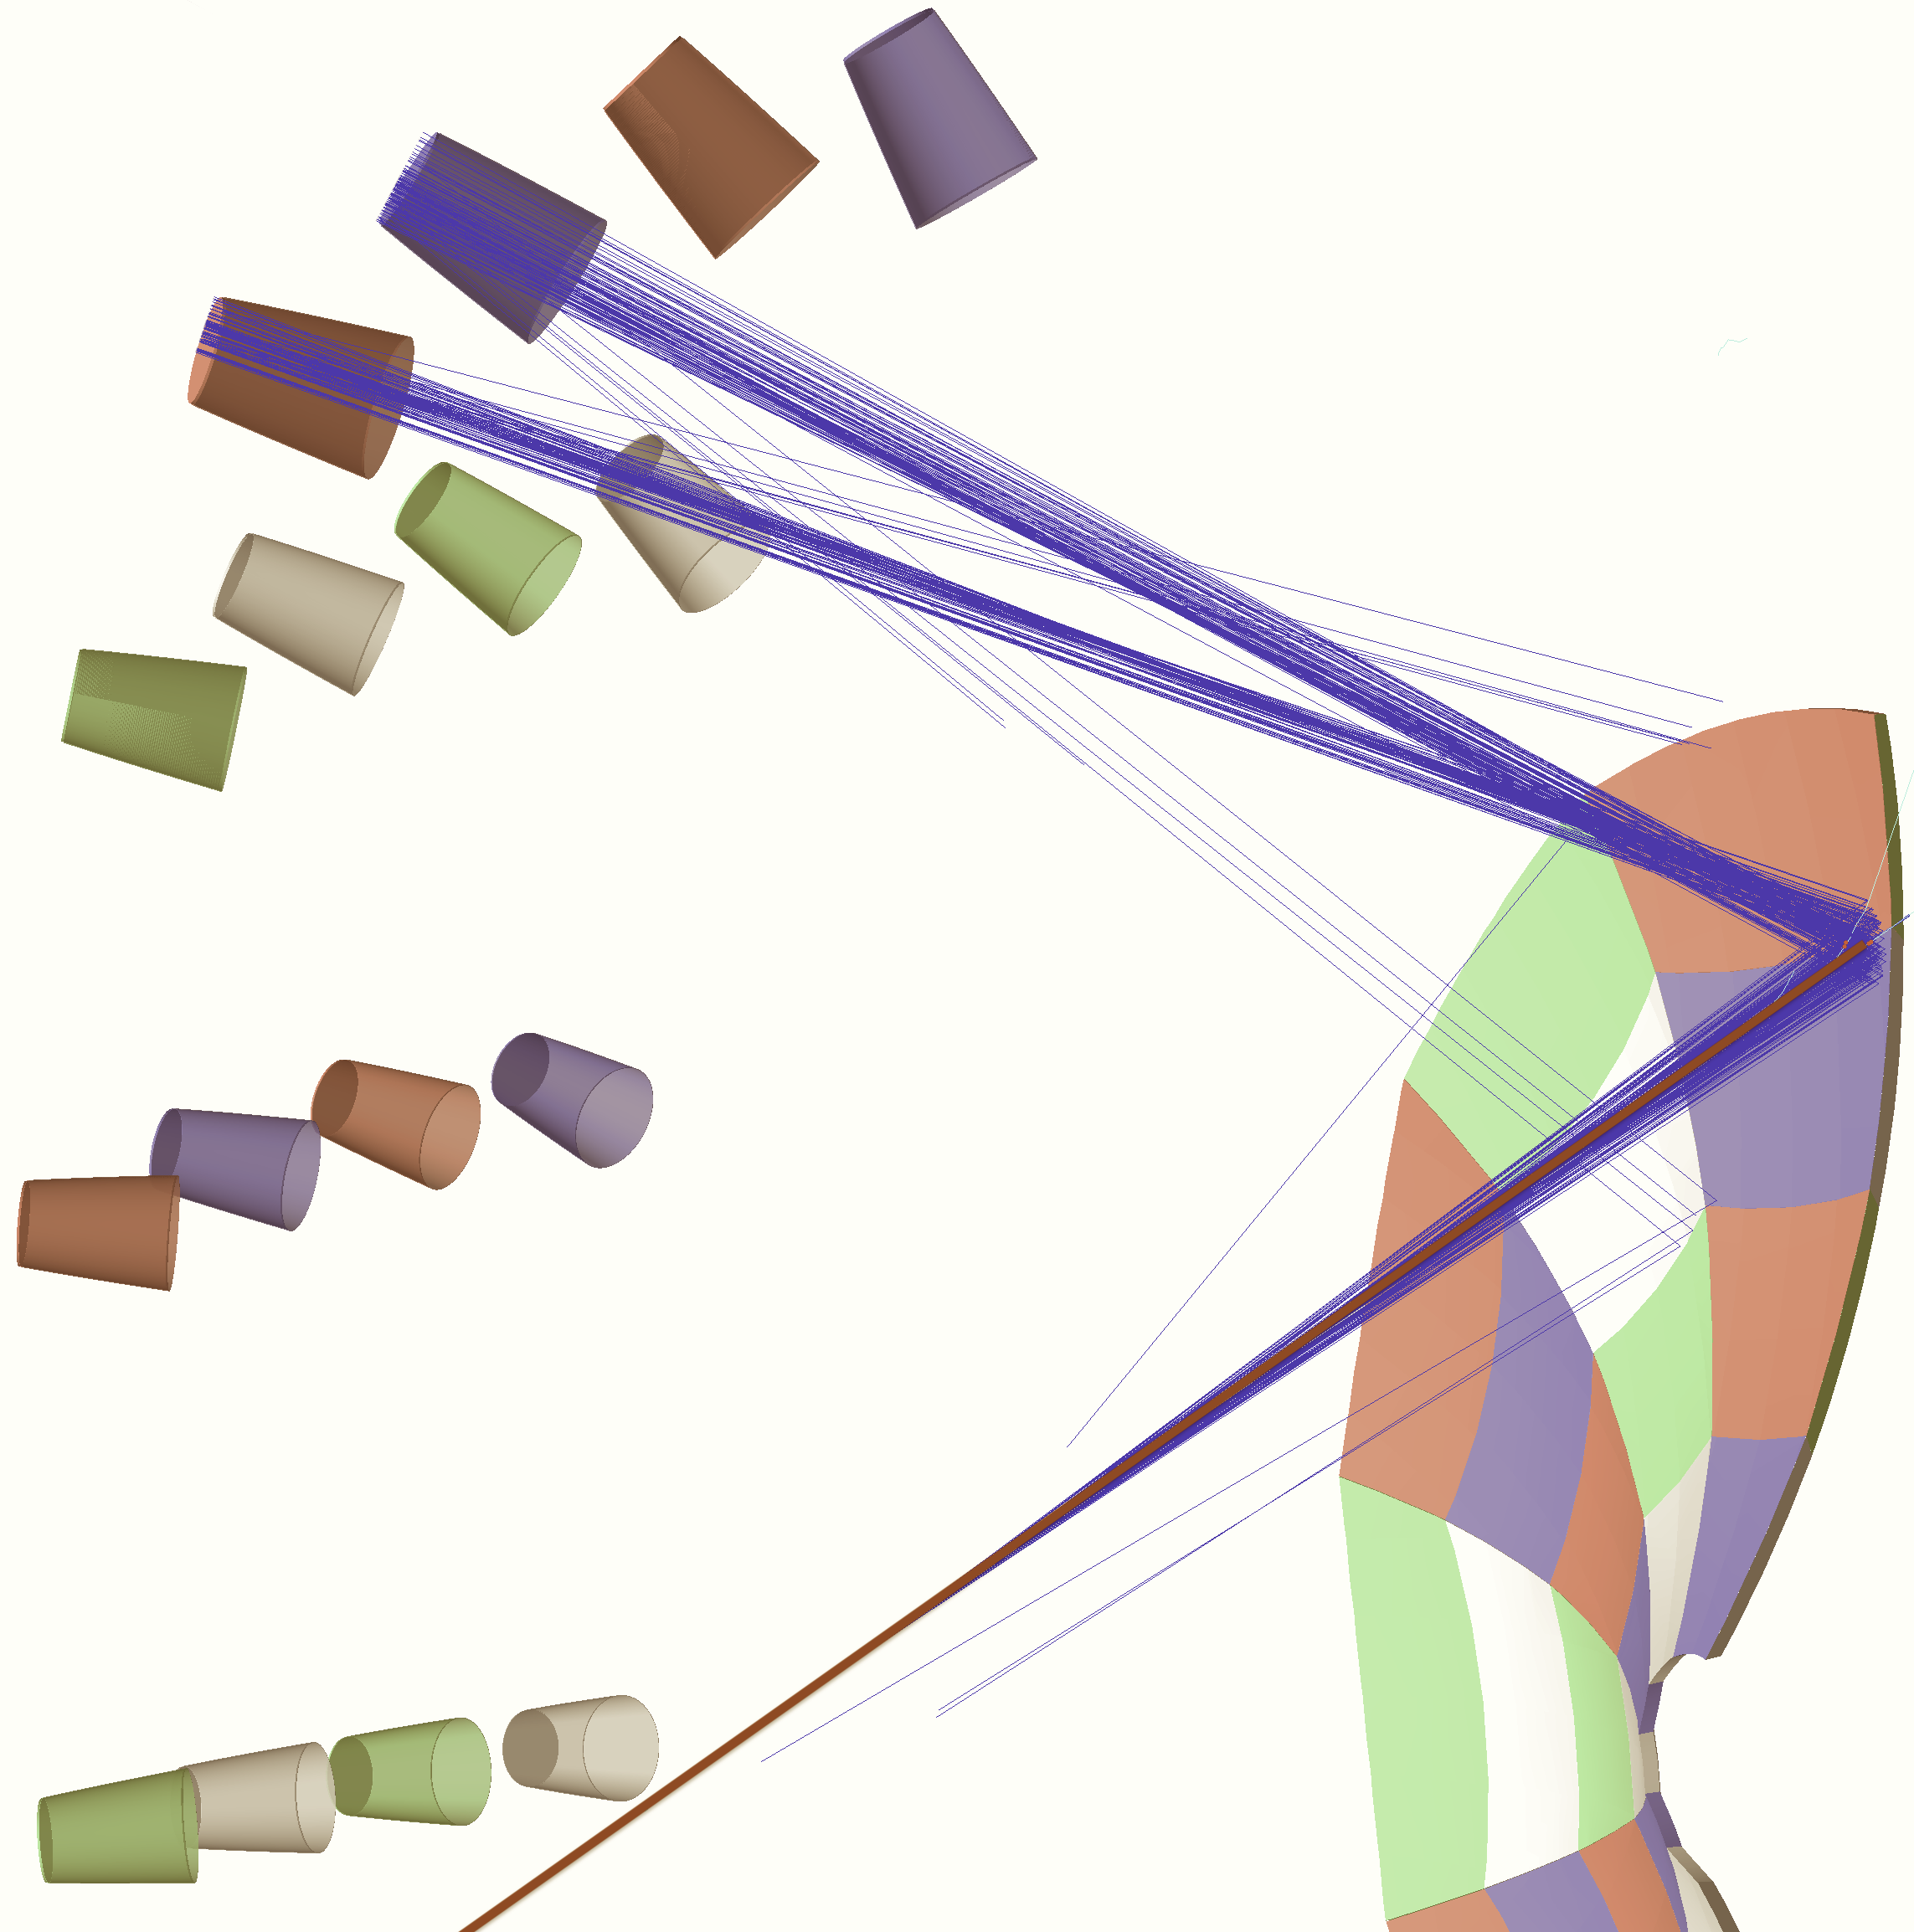
\includegraphics[width=0.99\columnwidth,keepaspectratio]{img/htccDetail.png}
	\caption{Top: the HTCC containment vessel. Bottom: an electron passing through the HTCC gas volume and emitting Cherenkov photons.
	         The light cone hits two mirrors and it is re-directed to the corresponding PMTs.}
	\label{fig:htccGeometry}
\end{figure}

\subsubsection{Digitization}
Photons that impinge on the PMT faces are processed with the digitization routine.
Each photon collected is input to the quantum efficiency algorithm at its wavelength to decide if it is finally detected.

The time average of all the photons is saved in the output after a time shift coming from the calibration database.
The digitized output bank variables are summarized in Table \ref{tab:htccBank}.

\begin{table}[h]
	\begin{center}
		\begin{tabular}{| c | c | c |}
			\hline \hline
			Variable  & Description                         \\
			\hline
             sector   &                   CLAS12 sector     \\
             ring     &                     theta index     \\
             half     &                     half-sector     \\
             nphe     &        number of photoelectrons     \\
             time     &         average time of the hit     \\
             hitn     &                      hit number     \\
			\hline \hline
		\end{tabular}
	\end{center}
	\caption{The digitized HTCC bank.}\label{tab:htccBank}
\end{table}

The time window  of the HTCC is set to 5 ns: all Geant4 steps within the same PMT and time window are collected in one hit.
